\documentclass[12pt,a4paper]{article}
\usepackage{apacite}
\usepackage{graphicx}
\usepackage{amsmath}
\usepackage{geometry}
\usepackage{setspace}
\usepackage{enumitem}
\usepackage{enumerate}
\usepackage{hyperref}
\usepackage{tabularx}
\graphicspath{ {./images/} }
\usepackage{lipsum} 


\geometry{margin=1in}
\setstretch{1.5}


\title{Optimizing Road Traffic Management with IoT-Based Road Traffic System with the use of Predictive Analytics and Cloud Computing }

\begin{figure}
    \centering
    
\includegraphics[width=.75\linewidth]{mmu2.jpg}
\end{figure}

\author{Group Members: \\
\textbf{RISHI ROOPEN (1231302892)} \\
\textbf{YOGAMITTRAN (1231302814)} \\
\textbf{IRFAN AHZA ZAKI (1231302448)} \\
\textbf{ADAM KAMAL (1231301368)} \\
\\
Course: CPT6123 Research Methodologies for Computer Science \\
\begin{figure}
    \centering
    \includegraphics[width=0.5\linewidth]{photo_2024-09-10_12-55-58.jpg}
    \caption{Enter Caption}
    \label{fig:enter-label}
\end{figure}
Assignment 2 - Research Proposal \\
Date of Submission: 25/9/2024}
\date{}

\begin{document}

\maketitle
\newpage

\tableofcontents
\newpage

\section{Executive summary }
    
    Traditional traffic management systems rely on fixed signal timings that are unable to adjust for changing traffic volumes. Congestion, delays, and a rise in fuel consumption follow from this. To change traffic management from a reactive to proactive approach predictive analytics to real-time and historical data can be applied. Delays are also caused by the fact that current infrastructures frequently find it difficult to handle the massive volumes of data generated by IoT sensors. By increasing data transfer speeds and processing efficiency, cloud computing provides a scalable answer to these problems. \\

This research attempts to create a predictive traffic management system to prevent the usage of traditional traffic management system by using Internet of Things (IoT) sensors and machine learning models such as Long Short-Term Memory (LSTM) networks, Convolutional Neural Networks (CNNs), and Density-Based Spatial Clustering of Applications with Noise (DBSCAN). Based on anticipated traffic patterns, the system will be built to proactively modify traffic signal timings. Furthermore, the integration of cloud computing technologies, namely Google Cloud and Amazon Web Services (AWS), will improve scalability and real-time data transfer.\\

The anticipated result of this research is predictive traffic management system that can minimize traffic jams, optimize signal timings, and use less fuel. The system can process real-time data more efficiently and can also scale to accommodate larger traffic systems by the integration of  cloud computing.  

\newpage



\section{Introduction}
Traditional traffic systems with fixed signal timings are unable to adjust to changing conditions, which causes delays and increased fuel consumption. Urban traffic congestion is a growing problem. Although real-time traffic data is provided by IoT sensors, most systems are reactive and only deal with issues after they occur. Although there are few practical uses for predictive analytics, it can forecast traffic and optimize signal timings using machine learning models like CNNs and LSTM.\\ 

Furthermore, the vast amount of data produced by IoT systems frequently surpasses the capability of conventional infrastructures, delaying real-time reactions. In order to process this data more effectively and ensure timely traffic management, cloud computing offers a scalable solution. In order to create a proactive traffic management system that lessens traffic, enhances flow, and uses less fuel, this research aims to integrate IoT, cloud computing, and predictive analytics. To prove the system's efficacy, real-world scenarios will be used for testing. 

\newpage

\section{Problem Statement with Justifications and Research Problems }\\

Current traffic management systems mostly rely on fixed signal timings. They are inefficient due to fluctuating traffic volumes causing congestion, delays, and increased fuel consumption. While IoT sensors provide real-time data, most of the time they operate reacting to real time traffic situation, failing to predict traffic conditions before congestion occurs. With predictive analytics using old and real-time data gather from IoT systems, this could change traffic management from reactive to proactive through prediction on future traffic. This approach would likely reduce congestion, travel times, and fuel consumption.\\

Although the IoT-based predictive systems have high potential, evidence on their effectiveness in larger scale is needed and most research is conducted through simulations or small-scale test environments, making the sort of data and result lacking. Without real-world test and example, the true effects of predictive analytics, such as congestion reduction and fuel efficiency improvements, remain doubted. It is important to do evaluation of the system's performance in real-world situation, using key indicators like travel time reduction and traffic density to provide insights of the effectiveness on optimizing traffic flow. \\

Another concern is real-time data transfer effectiveness for IoT-based traffic systems because of the large amounts of data from sensors on the road. Traditional infrastructures usually struggle with data processing speed and scalability, which cause more delays in traffic control responses. Cloud computing is deemed as one of the scalable solutions providing faster data processing and reducing latency. With cloud computing, IoT systems can manage larger data loads, ensuring more timely and efficient responses to traffic changes. This will also be a focus whether it can improve the real-time data transfer and scalability to make trafic management more responsive.

\newpage

\section{Research Questions, Hypothesis and Research Objectives}

\textbf{Research Question }
\begin{itemize}
    \item How to optimize Road Traffic Management with IoT-Assisted Road Traffic System using Predictive Analysis? 

    \item To what extent may predictive analysis be used to optimize Road Traffic Management with IoT-assisted Road Traffic System? 

    \item How can Real Time Data Transfer of IoT-Based Road Traffic System be enhanced using Cloud Computing? 
\end{itemize}
\textbf{Hypotheses }
\begin{itemize}
    \item IoT-Assisted Road Traffic System can optimize road traffic management better compared to standard practices. 

    \item Cloud computing can enhance real-time data transfer that is optimized through IoT-based system
\end{itemize}
\textbf{Objectives}
\begin{itemize}
    \item To develop a predictive traffic management system using IoT sensors. 

    \item To measure the effectiveness of predictive analytics in optimizing road traffic. 

    \item To enhance real-time data transfer for IoT-based systems using cloud computing. 
\end{itemize}

\newpage

\section{Literature Review Summary}

The Internet of Things (IoT) has revolutionized traffic management by introducing real-time data collection from sensors, vehicles, and traffic signals. It provides crucial insights and data into traffic conditions. This technology allows for more dynamic adjustments to traffic signals, helps manage congestion, and guides the transition from static systems to flexible, data-driven solutions (Khelifi \& Belouahri, 2022). \\ 

Urban traffic will become increasingly complex, hence why IoT-driven systems are necessary for optimizing traffic flow. However, even though traffic systems have advanced significantly with IoT, there is still a question of whether existing technologies fully answer modern traffic demands in large-scale urban environments. \\

\textbf{Predictive Analytics in Traffic Systems }\\

Predictive analytics enhances IoT-based traffic systems using historical and real-time data to predict future traffic congestion. Machine learning algorithms like Long Short-Term Memory (LSTM) networks and Convolutional Neural Networks (CNNs), help systems predict congestion and adjust signal timings cautiously, reducing any delays, fuel consumption, and environmental impact (Narayanan \& Shyamala, 2024). Although these models offer real-time adjustments, their effectiveness in larger-scale environments is still uncertain. Most studies have shown these benefits in small-scale tests but leave a gap in understanding their real-world application. \\

\textbf{Recent Developments in Machine Learning and IoT Integration }\\

Recent advancements in machine learning and IoT have further advanced traffic management capabilities. For example, ensemble learning models namely Decision Tree Regression and LSTM networks, combine historical and real-time data to forecast how the traffic flows and proactively adjust signals. By gathering the strengths of multiple algorithms, prediction accuracy will improve (Narayanan \& Shyamala, 2024).  \\

This integration of IoT with \textbf{Vehicle-to-Everything (V2X)} technology also plays an important role in enabling intelligent transportation systems (ITS). A three-layer architecture consisting of perception, communication, and application layers guarantees seamless data exchange and rapid responsiveness in managing traffic congestion (Dui et al., 2024). Despite these innovations, there is still a need for scalable solutions capable of handling larger traffic volumes in real time. \\

\textbf{Detection of Traffic Anomalies }\\

Detecting traffic anomalies is still considered a crucial challenge. \textbf{Density-Based Spatial Clustering of Applications with Noise (DBSCAN)} is a machine-learning algorithm that has been applied to cluster vehicles at intersections. This helps the systems in adapting traffic signals in real-time, therefore improving traffic flow and reducing delays by detecting sudden traffic surges (Shamitha et al., 2022). \\

However, the practical implementation of DBSCAN in highly congested urban areas presents challenges in terms of scalability and real-time processing capabilities. Current studies focus primarily on simulation environments, so field tests are necessary to validate DBSCAN’s real-time performance in urban traffic systems. \\

\textbf{Smart Signaling Systems and Cloud Computing }\\

IoT-assisted smart signaling systems that utilize real-time data from sensors and edge computing are created to make rapid adjustments to traffic signals. These systems adapt dynamically to changing traffic conditions, which improves road safety and reduces congestion. The use of cloud platforms for example AWS IoT has improved the scalability of these systems by providing real-time data analytics and management capacities (Saranya et al., 2024). \\ 

However, cloud computing can often lead to latency issues, especially when real-time decision-making is necessary. Therefore, cloud architectures are being researched to balance between real-time processing and the computational capacity of the cloud. (Dui et al., 2024). \\

\textbf{Challenges in Scalability and Real-Time Processing }\\

Despite the potential of these technologies, the trend of significant challenges is seen in all of them. Namely, scalability is a major issue, as the growing volume of data generated by IoT devices worries current systems. Distributed computing frameworks like Apache Hadoop and Spark, while effective for big data processing, are not yet fully optimized for real-time traffic systems (Khelifi \& Belouahri, 2022).  \\

Moreover, real-time data processing is still a challenge, as cloud-based architectures often have latency that prevents sub-second responses (Narayanan \& Shyamala, 2024). While edge computing has come up as a solution, the implementation in larger-scale systems requires further modification, particularly in distributed environments where fault tolerance is critical. \\

\textbf{Heterogeneous Data Integration and Machine Learning Optimization} \\

Another significant challenge is integrating heterogeneous data from multiple sources such as sensors, GPS, and cameras. Making sure communication is seamless between devices using multiple protocols requires advanced techniques in data fusion and interoperability (Shamitha et al., 2022).\\  

Furthermore, it is still a challenge to optimize machine learning algorithms like LSTM and CNN-LSTM for real-time applications due to their computational resource demands. Current research focuses on model compression techniques such as pruning and quantization to make these algorithms more viable for real-time, resource-constrained environments (Khelifi \& Belouahri, 2022). \\

\newpage

\textbf{Fault Tolerance and Reliability }\\

Fault tolerance and reliability are also critical concerns in distributed traffic management systems. Failures in sensors, communication links, or processing nodes can brutally mess up traffic management. To reduce these risks, redundancy techniques and self-healing algorithms are being developed to maintain system functionality even in situations where the components fail (Saranya et al., 2024). It is also still an issue to ensure that these fault-tolerant systems can scale to handle the vast data volumes produced by urban traffic environments. \\

\textbf{Linking the Literature to Research Gaps} \\

As these technologies have made significant progress in traffic management, several key gaps remain. The first research question, "How to optimize Road Traffic Management with IoT-Assisted Road Traffic Systems using Predictive Analysis?", addresses the shift from reactive to proactive traffic management. The literature reveals that while predictive models like LSTM and DBSCAN are promising, their real-world effectiveness in large urban environments is yet to be comprehensively tested (Narayanan \& Shyamala, 2024; Shamitha et al., 2022). \\

The research question "To what extent can predictive analysis optimize Road Traffic Management with IoT-Assisted Road Traffic Systems?" aims to analyze the scalability and efficiency of predictive models in resource-constrained environments. Recent studies mainly only focus on small-scale implementations, leaving a gap and insight in understanding their capabilities in larger, real-world settings (Khelifi \& Belouahri, 2022). \\

The final research question dwells on the enhancement of real-time data transfer in IoT-based road traffic systems using cloud computing. The purpose is to explore how cloud models can effectively address data transmission bottlenecks. Even though these models have the potential to improve the scalability and data processing efficiency, it is still needed to do further research to address latency issues in real-time applications (Saranya et al., 2024; Dui et al., 2024). \\

\textbf{Conclusion }\\

While focusing on gaps and challenges in IoT-based traffic management systems, this research will explore the integration of predictive analytics and cloud computing. By using and gaining insight from predictive models such as LSTM and DBSCAN and investigating the application of cloud architectures on real-time data transfer, this study tries to find solutions to the growing complexities of urban traffic management. While current technologies are quite advanced, further research is still required to make sure these systems can operate on a larger scale effectively in real-world environments. 
 
\cite{10384717}, \cite{10568678}, \cite{10575594}, \cite{9914294}, \cite{9931585}

\newpage

\section{Research Methodology }

This project consists of the following main components: \\

\textbf{PART A:} A predictive traffic management system using IoT sensors \\

\textbf{PART B:} Measure the effectiveness of predictive analytics in optimizing road traffic.\\

\textbf{PART C:} Enhancing Real Time Data Transfer with Cloud Computing.\\ 

\textbf{PART D:} Results Analysis.\\

\subsection{PART A: A predictive traffic management system using IoT sensors }


The development of the new traffic management system is as shown in the Figure. 

\begin{figure}[h]
    \centering
    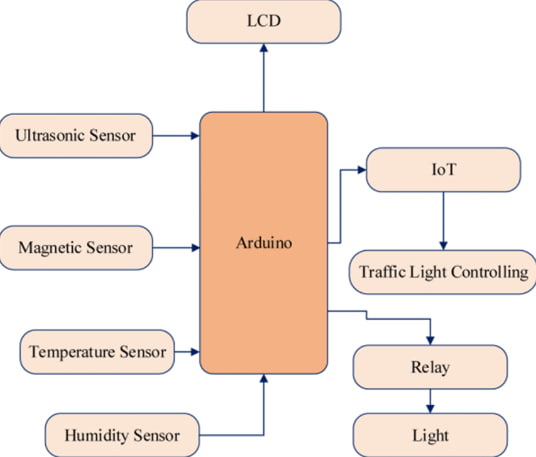
\includegraphics[width=0.5\linewidth]{photo_2024-09-25_10-58-21.jpg}

\end{figure}

The system design and architecture involves a four-layer design as done in Shamita.C et al. (2022), G.Saranya et al. (2024) and Hongyan Dui et al. (2024) which involves the need to gather, process and analyse real-time traffic data using IoT sensors:

\begin{itemize}
    \item Sensing Layer: Includes all necessary instruments such as ultrasonic, magnetic and environmental sensors 

    \item Communication Layer: Uses MQTT protocols for communication between firmware 

    \item Processing Layer: Cloud-based infrastructure used for data management such as AWS 

    \item Control Layer: Utilizing machine learning models to adjust and control signal timings  
\end{itemize}

The implementation of \textbf{Predictive Model Development} is as follows:

\begin{itemize}
    \item Machine Learning Algorithm DBSCAN (Density-Based Spatial Clustering of Applications with Noise) is used for detection of anomalies in traffic flow and clustering of high-traffic areas based on real-time data feed featured in Shamita.C et al. (2022). 

    \item The use of Long Short-Term Memory (LSTM) networks and Convolutional Neural Networks (CNNs) is also implemented to allow traffic systems to predict congestion and optimize signal timings proactively. 
\end{itemize}

Implementation of \textbf{Control Algorithms}: 

\begin{itemize}
    \item An adaptive traffic light control is implemented using data driven decision making allowing the machine learning algorithm to perform linear regression for predicting traffic density and reinforcement learning also seen in G.Saranya et al. (2024) and Hongyan Dui et al. (2024). 

    \item With the use of \textbf{Ensemble learning models}, which combine algorithms like Decision Tree Regression and LSTM networks. As noted by Narayanan \& Shyamala (2024), these models leverage both historical and real-time data to forecast traffic flow and adjust signals dynamically, reducing congestion and wait times 
\end{itemize}

The system will undergo simulation and testing using real-time traffic data. MATLAB simulator will used to model traffic conditions and to measure the system's performance under varying traffic volumes 

\subsection{PART B: Measure the effectiveness of predictive analytics in optimizing road traffic.}



 The effectiveness of the model will be validated by comparing its prediction to real-time traffic data. Accuracy, latency and system efficiency will be the main priority in evaluating the performance of the system as done in Hongyan Dui et al. (2024). 

The systems performance will be evaluated using suitable metrics as follows:

\begin{itemize}
    \item Traffic Flow Rate (vehicle per minute): Volume of traffic passing through an intersection. 

    \item Congestion Level Reduction (\%): The system’s ability to reduce congestion during peak hours 

    \item Average Delays per Vehicle (s): Vehicle waiting time at traffic lights 

    \item System Responsiveness (ms): Time taken for system to react 

    \item Prediction Accuracy (\%): Accuracy of machine learning model ability to predict future traffic conditions 

    \item Throughput (vehicle per hour): Number of vehicles passing through a specific intersection at a given period 
\end{itemize}

The system will be tested across multiple real-world scenarios such as: 

\begin{itemize}
    \item Peak Hour Traffic: Test the model’s ability to optimize flow of traffic during high congestion period 

    \item Accident Scenarios: Assess how the system reroutes traffic and adapts to unplanned disruption 
\end{itemize}

Multi-Intersection Coordination: Evaluate the capability of the model to handle multiple intersections, improving overall urban traffic management. 

\newpage

\subsection{PART C: Enhancing Real Time Data Transfer with Cloud Computing }

The Cloud Computing to Enhance Real Time Data Transfer design is as follow in the Figure:

\begin{figure}[h]
    \centering
    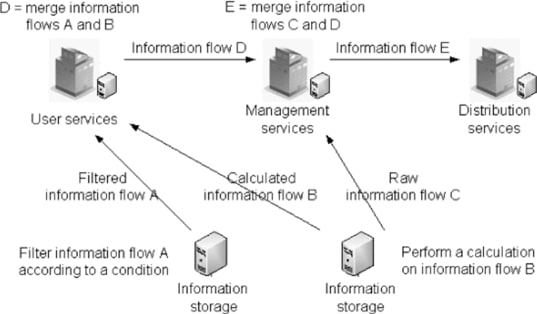
\includegraphics[width=0.5\linewidth]{photo_2024-09-25_11-13-11.jpg}

\end{figure}

The infrastructure of the system consists of tools such as: 

\begin{itemize}
    \item Amazon Web Services (AWS)  

    \item Google Cloud  

    \item Azure
\end{itemize}

This allows for \textbf{}Infrastructure-as-a-Service (IaaS) and \textbf{Platform-as-a-Service (PaaS)} to manage real-time data from IoT devices. \\

The process of Data Transfer and Processing of information is managed through the use of \textbf{Message Queuing Telemetry Transport (MQTT)} and \textbf{HTTP/2 cloud services} for ultralightweight communication between devices and cloud servers as used in G.Saranya et al. (2024). The use of Streaming Analytics such as Amazon Kinesis and Apache Spark will be integrated to allow quick process and analysation of real-time data as it arrives to the cloud as done in Rohit Ranchal et al. (2020). \\

For storage of large volumes of data that is intended to be processed in real time, cloud-based storage services such as Amazon S3 or Azure Blob will be used as in G.Saranya et al. (2024). \\

The system is intended to follow a distributed data model architecture, where data from multiple sources is processed in parallel across different cloud regions which allows for better load balancing and latency as used in G.Saranya et al. (2024) \\

Type of Algorithms used may include: 

\begin{itemize}
    \item Load Balancing Algorithm 

    \item Compression Algorithm 

    \item Encryption Algorithm 
\end{itemize}

The systems performance will be evaluated using suitable metrics as follows:

\begin{itemize}
    \item \textbf{Latency (ms):} Measures the time taken for data to be transmitted from the source to the sources the cloud back 

    \item \textbf{Throughput (Mbps):} Evaluates the rate at which data is successfully transmitted through the cloud 

    \item \textbf{Scalability:} Assesses the ability for the system to scale up or down based on the number of connected devices and the volume of data being transferred 

    \item \textbf{Cost Efficiency:} Compares cost of data transfer of different cloud-based systems
\end{itemize}

\subsection{PART D: Results Analysis}

 

Finally, all the results obtained will be analysed and benchmarked from the information gathered and all insights will be documented from the experiments conducted.
\newpage

\section{Research Activities and Milestones}

\begin{table}[h]
    \centering
\begin{tabularx}{1.1\textwidth} { 
  | >{\raggedright\arraybackslash}X 
  || >{\raggedright\arraybackslash}X
  | >{\raggedright\arraybackslash}X
  | >{\raggedright\arraybackslash}X
  | >{\raggedright\arraybackslash}X
  |} 
 \hline
 
Phase & Objective & Activities & Milestones & Timeline \\ 
\hline
\hline
1. Literature Review and Conceptualization & Gather foundational knowledge on IoT, predictive analytics, and traffic management systems & - Conduct critical literature review.\newline
- Identify gaps and challenges.\newline
- Develop research questions and hypotheses.s & - Completion of literature review.\newline
- Finalized research questions and objectives. & Weeks 1-8 \\ 
\hline
2. System Design and Development & Design a predictive traffic management system using IoT sensors and cloud computing & - Design a four-layer IoT-based architecture.\newline
- Develop predictive models (DBSCAN, LSTM/CNN).\newline
- Set up cloud infrastructure. (AWS, Google Cloud) & - Completion of system design.
- Initial implementation of models.\newline
- Cloud infrastructure setup. & Weeks 9-20 \\ 
\hline
3. Simulation and Testing & Test the system using real-time traffic data simulations & - Simulate traffic conditions.\newline
- Test system response to various scenarios.\newline
- Measure system effectiveness. (e.g., flow rate, delays, responsiveness)& - Completion of simulation setup.\newline
- Initial performance data collected.\newline
- Model refinements. & Weeks 21-30 \\ 
\hline
\end{tabularx}
\end{table}
\newpage

\begin{table}[h!]
    \centering

\begin{tabularx}{1.1\textwidth}
{ 
  | >{\raggedright\arraybackslash}X 
  || >{\raggedright\arraybackslash}X
  | >{\raggedright\arraybackslash}X
  | >{\raggedright\arraybackslash}X
  | >{\raggedright\arraybackslash}X
  |} 
 \hline
 4. Real-World Data Integration and Optimization & Validate and optimize the system with real-world traffic data & - Collect real-world traffic data.\newline
- Fine-tune machine learning models.\newline
- Optimize latency and scalability using cloud services. & - Successful real-world data integration.
- System optimized.\newline
- Latency/scalability improvements. & Weeks 31-42 \\ 
\hline
5. Evaluation and Analysis & Evaluate system performance and draw conclusions & - Analyze simulation and real-world data.\newline
- Compare system performance to baseline systems.\newline
- Document system effectiveness and findings. & - Performance evaluation report.\newline
- System improvements identified. & Weeks 43-48 \\ 
\hline
6. Final Report and Presentation & Summarize research findings and present & - Compile final research results.\newline
- Prepare final report and presentation of research, design, testing, and findings. & - Submission of final report.\newline
- Research presentation completion. & Weeks 49-52 \\ 
\hline
\end{tabularx}
\end{table}

\newpage

\section{Expected Results and Impact}
\begin{itemize}
    \item \textbf{Expected Results and Findings }
    \begin{itemize}
        \item A predictive traffic management system using IoT sensors 

        \item An enhanced real-time data transfer using cloud computing 
    \end{itemize}
    \item \textbf{Impact of the research on society, nation and/or economy}
    \begin{itemize}
        \item As Malaysia is car-centric nation, the significant findings in this research will benefit the future urban development of the nation by reducing traffic congestion and improving road safety. As Malaysia aligns its interest towards smart cities as the more superior form of city development, the findings will assist in contributing towards the support of the development. 

        \item With the boosts of productivity and reduced cost of fuel spending thanks to efficient traffic management, this will provide a significant boost towards the economy 

        \item Through the enhancement of real-time data transfer via cloud computing, the improvement towards access of information and advance healthcare through telemedicine will accelerate national goal of digital transformation and enhances critical infrastructure required for better management of data. 

        \item With these advancements in IoT and cloud computing a significant stride towards computer science will be represented with the contribution towards a more efficient and technologically advanced society and economy. 
    \end{itemize}
\end{itemize}

% References
\newpage
\bibliographystyle{apacite} % Choose the appropriate bibliography style (e.g., APA, IEEE)
\bibliography{MyBib} % Make sure to include a MyBib.bib file with your references

\end{document}


